\chapter{Automata Theory}

\textit{Automata theory} is the study of \textit{automata} and their behavior. An \textit{automaton} is a self-operating machine designed to follow or respond to a predetermined sequence of operations. Automata include physical devices such as cuckoo clocks, mechanical watches, robots, and computer processors as well as \textit{abstract machines}. An abstract machine is any formal description of \textit{mechanical behavior}. An abstract machine that is used to formally describe computation is called a \textit{model of computation}. This is a mathematical description of what a computer is, and it models the computation that a real, concrete computer could actually perform, if you were to implement that computer according to the model's specifications. Like their concrete counterparts, abstract machines have \textit{state}, a set of information in the \textit{present} that was acquired due to \textit{past} events. All automata begin with a \textit{starting state}, receive some sort of \textit{input}, and \textit{transition} to another state based on the value of that input and the value of its current state. \\

One \textit{abstract automaton} in particular fully models not only the computation that is performed by today's state-of-the-art computers, but also the very process of computation itself. We will spend a lot of time in this guide discussing the structure and behavior of this model as well as what its limitations imply regarding the future of computing, software, mathematics, and the meaning of life. We will also briefly explore the abstract automata that exist in pure mathematics and model computation that is not physically realizable. \\

\section{From Knots to Nodes}

It is worth pausing here to think about what the word \textit{node} really means. It comes from the Latin word \textit{nodus}, which means \textit{knot}. A node is like a knot in a string: a distinguishable lump at a certain position. And between any two adjacent knots in a string, there is a \textit{link} \dots\ of string. Similarly, between any two adjacent links, there is a knot. \\

The knots and the links cannot exist independent of each other. Without knots, there are no links of string---just one, continuous string. Without links, knots are totally unanchored and have no sense of position. Now, one could argue that a single knot is sufficient for the existence of links in a string, but such a view is naive and presumes a familiar, everyday sort of string. \\

For example, yes, you can tie a single knot in a shoelace, and you might then call the floppy bits on either side of it "links." But when you call something like this a link, what you are really pointing out is its \textit{finite length}. That is, the "string link" \textit{starts} at the knot and \textit{ends} at the tip of the aglet. But length is a nonessential detail for links---the essence of a \textit{link} is its \textit{connecting} of things. A better term in this case would be \textit{loose end} or simply \textit{end}. A knot with two loose ends is shown below: \\

\begin{center}  
    \begin{tikzpicture}[scale=0.2]
        \begin{knot}[
            consider self intersections,
            flip crossing=2
            clip width=5,
        ]
            \strand[ultra thick]
                (90:1.25) to[out=180,in=-120,looseness=2]
                (-30:1.25) to[out=60,in=120,looseness=2]
                (210:1.25) to[out=-60,in=0,looseness=2] (90:1.25);
        \end{knot}
        
        \draw [ultra thick, dashed] (-1.2,0) -- ++(-5,0);
        \draw [ultra thick, dashed] (1.2,0) -- ++(5,0);
    \end{tikzpicture}
\end{center}

For our purposes, it is better to envision a taut string that stretches to infinity in both directions and to think of a \textit{link} as a \textit{connector of a knot pair} whose length may or may not be important. With this model, there must be at least two knots in the string if we are to think of them as \textit{nodes} (i.e. things that are connected to something else). A string with five \textit{trefoil} (three-leafed) knots and four links is shown below: \\

\begin{center}
    \begin{tikzpicture}[scale=0.2]
        \foreach \x in {-2,-1,0,1,2} {
            \begin{knot}[
                consider self intersections,
                flip crossing=2
                clip width=5,
                xshift=\x*250,
            ]
                \strand[ultra thick]
                    (90:1.25) to[out=180,in=-120,looseness=2]
                    (-30:1.25) to[out=60,in=120,looseness=2]
                    (210:1.25) to[out=-60,in=0,looseness=2] (90:1.25);
            \end{knot}
        }
        
        \foreach \x in {-1,0,1,2} {
            \draw [ultra thick] (-1.2+\x*8.75,0) -- ++(-6.45,0);
        }
        \draw [ultra thick, dashed] (-18.75,0) -- ++(-9,0);
        \draw [ultra thick, dashed] (18.75,0) -- ++(9,0);
    \end{tikzpicture}
\end{center}

In the mathematical field of \textit{knot theory}, knots are defined similarly, but they do not have ends. That is, a mathematical knot is defined as a \textit{closed} circle embedded in a three-dimensional Euclidean space and subject to continuous deformation. Essentially, this means that you can cut a circular string at a point, tangle it, and close the circle at the same point to form any mathematical knot you like. The process of tying a \textit{cinquefoil}, a knot with five \textit{crossings}, is given below as an example: \\[\baselineskip]

\resizebox{\textwidth}{!}{
    \begin{tikzpicture}
        \draw[very thick] (0,0) circle (2);
        \filldraw[line width=1mm,textbook-blue] (0,0) ++(60:2) arc (60:70:2);
        
        \begin{knot}[
            consider self intersections,
            flip crossing=2
            clip width=5,
            xshift=150
        ]
            \strand[very thick] (2,0) .. controls +(0,1.0) and +(54:1.0) .. (144:2) .. controls +(54:-1.0) and +(18:-1.0) .. (-72:2) .. controls +(18:1.0) and +(162:-1.0) .. (72:2);
        \end{knot}
        
        \begin{knot}[
            consider self intersections=true,
            %  draft mode=crossings,
            flip crossing/.list={2,4},
            only when rendering/.style={
            %    show curve controls
            },
            xshift=300
        ]
            \strand[very thick] (2,0) .. controls +(0,1.0) and +(54:1.0) .. (144:2) .. controls +(54:-1.0) and +(18:-1.0) .. (-72:2) .. controls +(18:1.0) and +(162:-1.0) .. (72:2) .. controls +(162:1.0) and +(126:1.0) .. (-144:2);
        \end{knot}
        
        \begin{knot}[
            consider self intersections=true,
            %  draft mode=crossings,
            flip crossing/.list={2,4},
            only when rendering/.style={
            %    show curve controls
            },
            xshift=450
        ]
            \strand[very thick] (2,0) .. controls +(0,1.0) and +(54:1.0) .. (144:2) .. controls +(54:-1.0) and +(18:-1.0) .. (-72:2) .. controls +(18:1.0) and +(162:-1.0) .. (72:2) .. controls +(162:1.0) and +(126:1.0) .. (-144:2) .. controls +(126:-1.0) and +(0,-1.0) .. (2,0);
        \end{knot}
    \end{tikzpicture}
} \\[\baselineskip]

Note that because mathematical knots are closed, they cannot be linked together like knots in a string. Instead, a link in knot theory is a collection of knots that are knotted together. \\

\section{Concrete and Abstract Machines}

Let's take a simple, concrete machine and try to visualize the abstract machine that underlies it. Consider a cuckoo clock. Every day, at noon, a small plank with a mechanical bird perched on its lip will extend from a hole above the clock face, powered by a working motor. Once the plank is fully extended, the bird will flap its metal wings and maybe turn its head as a song is played from a revolving music box inside the clock. Then, when it is 12:01 PM, the music will stop, the bird will still, and the plank will retract. The process will occur again the next day, at noon. \\

The machine's components here are the plank, the bird, and the music box. The components each have two states: the plank can be retracted or extended, the bird can be still or flapping its wings, and the music box can be paused or playing. The input to this machine is whether or not the clock hands both point straight at 12. We can say that this automaton has a state that can be expressed in terms of the states of its components. We can represent its starting state with the sequence (0,0,0) (i.e. the plank is retracted, the bird is still, and the music box is paused). The automaton can receive one of two inputs, 1 or 0 (i.e. both clock hands point straight at 12 or they do not). This input might be implemented with an electromechanical switch that turns the motor on or off.

\paragraph{(0,0,0) -> (1,0,0)} We start at state (0,0,0). As the morning passes, the automaton receives a constant input of 0, which keeps it in its starting state. At noon, the input switches to 1, and the automaton transitions to the state (1,0,0). As the plank extends and transitions its own state from 0 to 1, the bird remains still, and the music box remains paused. Once the plank is fully extended, we are in state (1,0,0).

\paragraph{(1,0,0) -> (1,1,1)} We expect that the plank will be fully extended well before 12:01 PM, so the input should still be 1. However, if for some reason the input is 0, we should transition back to (0,0,0), as the machine should only operate outside of its starting state between 12:00 and 12:01 PM. This is a simple example of \textit{strange input}. The input 0 at this state is unexpected, but it is technically possible. It is a better idea to define the behavior for this unexpected case, rather than to allow the input to cause unexpected behavior. On the other hand, if the input is 1 at this state, the automaton transitions to the state (1,1,1). The plank is fully extended, the bird is flapping its wings, and the music box is playing.

\paragraph{(1,1,1) -> (0,0,0)} Before 12:01 PM, the input is still 1, and that input should keep the automaton in its current state of (1,1,1). When 12:01 PM rolls around, the input will now be 0. In this case, we would like to return to the original state. On receipt of the input 0 while in state (1,1,1), the automaton transitions back to its starting state, (0,0,0). This abstract machine is shown below with a state format of (plank, bird, music) and an input specifying if the clock hands point exactly toward 12.

% Drawing of "Bad Automaton"
\begin{center}
    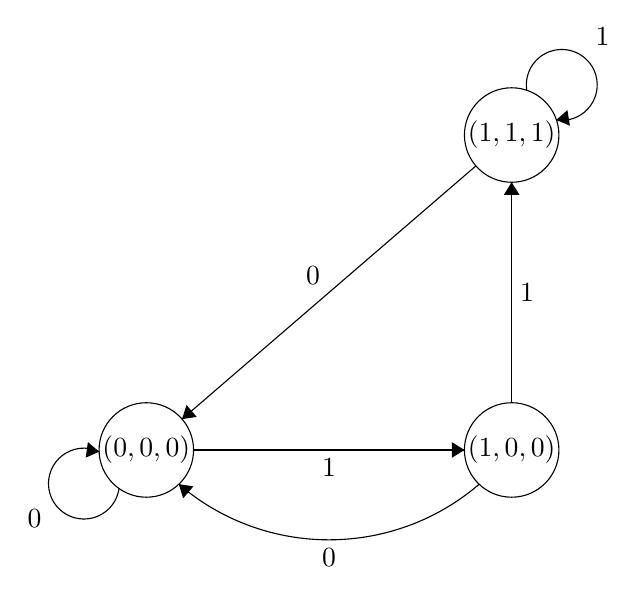
\begin{tikzpicture}[scale=0.2]
        \tikzstyle{every node}+=[inner sep=0pt]
        \draw [black] (28.4,-36.5) circle (3);
        \draw (28.4,-36.5) node {$(0,0,0)$};
        \draw [black] (51.6,-36.5) circle (3);
        \draw (51.6,-36.5) node {$(1,0,0)$};
        \draw [black] (51.6,-16.5) circle (3);
        \draw (51.6,-16.5) node {$(1,1,1)$};
        \draw [black] (31.4,-36.5) -- (48.6,-36.5);
        \fill [black] (48.6,-36.5) -- (47.8,-36) -- (47.8,-37);
        \draw (40,-37) node [below] {$1$};
        \draw [black] (51.6,-33.5) -- (51.6,-19.5);
        \fill [black] (51.6,-19.5) -- (51.1,-20.3) -- (52.1,-20.3);
        \draw (52.1,-26.5) node [right] {$1$};
        \draw [black] (26.668,-38.935) arc (-7.69924:-295.69924:2.25);
        \draw (21.78,-40.87) node [left] {$0$};
        \fill [black] (25.41,-36.61) -- (24.69,-36) -- (24.55,-36.99);
        \draw [black] (49.539,-38.673) arc (-49.35642:-130.64358:14.645);
        \fill [black] (30.46,-38.67) -- (30.74,-39.57) -- (31.39,-38.81);
        \draw (40,-42.71) node [below] {$0$};
        \draw [black] (52.56,-13.67) arc (189:-99:2.25);
        \draw (56.9,-10.25) node [right] {$1$};
        \fill [black] (54.43,-15.54) -- (55.3,-15.91) -- (55.14,-14.92);
        \draw [black] (49.33,-18.46) -- (30.67,-34.54);
        \fill [black] (30.67,-34.54) -- (31.6,-34.4) -- (30.95,-33.64);
        \draw (38.99,-26.01) node [above] {$0$};
    \end{tikzpicture}
\end{center}
\vspace{5mm}

This is a perfectly reasonable abstract machine, but something isn't right. It does not accurately simulate the behavior of the cuckoo clock we described. What happens when the clock strikes midnight? The clock hands will point at 12, producing an input of 1, but we don't want the bird to wake everyone up at midnight. We could use two bits of input: whether or not the hands are between 12:00 and 12:01, and whether it is AM or PM. Additionally, the music never plays unless the bird is flapping its wings, so we can combine those states. The abstract machine is better represented by the diagram below with a state format of (plank, bird/music) and an input format of (hands are toward 12, is PM).

% Drawing of "Good Automaton"
\begin{center}
    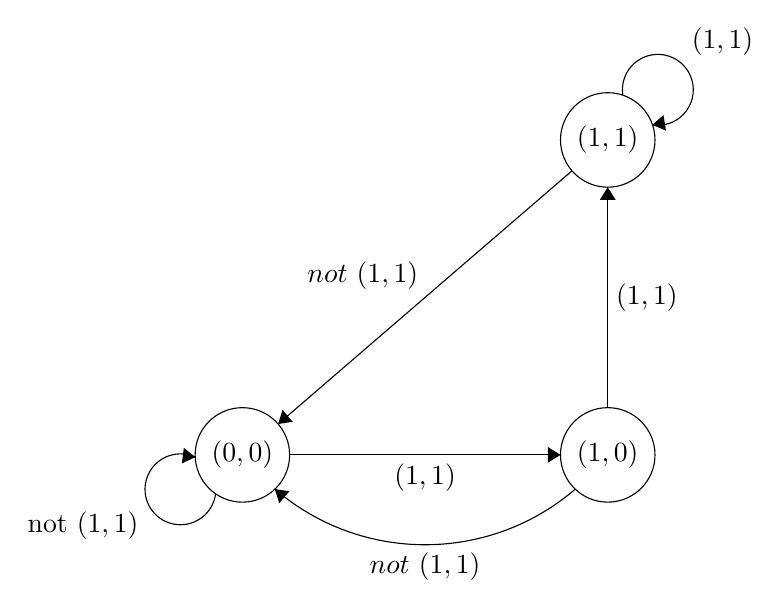
\begin{tikzpicture}[scale=0.2]
        \tikzstyle{every node}+=[inner sep=0pt]
        \draw [black] (28.4,-36.5) circle (3);
        \draw (28.4,-36.5) node {$(0,0)$};
        \draw [black] (51.6,-36.5) circle (3);
        \draw (51.6,-36.5) node {$(1,0)$};
        \draw [black] (51.6,-16.5) circle (3);
        \draw (51.6,-16.5) node {$(1,1)$};
        \draw [black] (31.4,-36.5) -- (48.6,-36.5);
        \fill [black] (48.6,-36.5) -- (47.8,-36) -- (47.8,-37);
        \draw (40,-37) node [below] {$(1,1)$};
        \draw [black] (51.6,-33.5) -- (51.6,-19.5);
        \fill [black] (51.6,-19.5) -- (51.1,-20.3) -- (52.1,-20.3);
        \draw (52.1,-26.5) node [right] {$(1,1)$};
        \draw [black] (26.699,-38.957) arc (-6.96472:-294.96472:2.25);
        \draw (21.83,-40.98) node [left] {not $(1,1)$};
        \fill [black] (25.42,-36.64) -- (24.68,-36.05) -- (24.56,-37.04);
        \draw [black] (49.539,-38.673) arc (-49.35642:-130.64358:14.645);
        \fill [black] (30.46,-38.67) -- (30.74,-39.57) -- (31.39,-38.81);
        \draw (40,-42.71) node [below] {$not\mbox{ }(1,1)$};
        \draw [black] (52.56,-13.67) arc (189:-99:2.25);
        \draw (56.9,-10.25) node [right] {$(1,1)$};
        \fill [black] (54.43,-15.54) -- (55.3,-15.91) -- (55.14,-14.92);
        \draw [black] (49.33,-18.46) -- (30.67,-34.54);
        \fill [black] (30.67,-34.54) -- (31.6,-34.4) -- (30.95,-33.64);
        \draw (36.05,-26.01) node [above] {$not\mbox{ }(1,1)$};
    \end{tikzpicture}
\end{center}
\vspace{5mm}

Note that the actual complexity of the concrete cuckoo clock would be a bit more complicated than the automaton above. For example, what does the bird do specifically when it is on? Perhaps it raises and lowers its wings three times, turns its head to the right twice, and repeats. This process can be modeled by a different automaton. To fully model a concrete automaton, we must reduce it to an abstract machine, a system of states and transitions that account for every intended behavior. Abstract machines are capable of modeling systems of any arbitrary complexity. The automaton above is a model of computation called a \textit{finite-state machine} (FSM), and it will be the first abstract machine that we will discuss.
\\

\section{Formalization of an Abstract Machine}

\begin{tcolorbox}[breakable, enhanced, colback=textbook-blue, sharp corners]
    \vspace{3mm}
    \begin{center}
        \textbf{A Brief Introduction to Formal Grammars}
    \end{center}

    A formal grammar is a finite set of \textit{production rules} that specifies what a particular language is supposed to look like. It formalizes the structure of "grammatical units" in a language. This is done in order to enforce a specific alphabet, a consistent lexicon, and a predictable sentence structure, all of which contribute to how useful and distinct any given language is. \\
        
    A grammar $G$ consists of the following components:
    \begin{itemize}
        \item A finite set $N$ of \textit{nonterminal} symbols.
        \item A finite set $\Sigma$ of \textit{terminal} symbols that is disjoint from $N$.
        \item A symbol $S\in N$, designated as the \textit{start symbol}.
        \item A finite set $P$ of \textit{production rules} where each rule is of the form ${(\Sigma\cup N)^*N(\Sigma\cup N)^*\rightarrow(\Sigma\cup N)^*}$.
    \end{itemize}
        
    Put another way, a production rule converts a sequence of symbols to another sequence of symbols. If a rule is of the form \textit{left-hand side $\rightarrow$ right-hand side}, each side can contain terminals and nonterminals, but its left-hand side must contain at least one nonterminal. A nonterminal is a symbol that is replaced by other symbols when an appropriate rule is applied. Unlike a terminal, it does not belong to the alphabet of the language, but rather represents a sequence of symbols that do. Terminals cannot be replaced by other symbols once chosen. \\
        
    Let's construct a simple formal grammar. It is typical for the nonterminals to be uppercase and for the terminals to be lowercase. Let $N=$ \{SENTENCE, NOUN, ADJ\}, $\Sigma=$ \{the, dog, building, plays, fluffy, good\}, and $S=$ SENTENCE. The rules of $P$ are given below.
        
    \begin{itemize}
        \item SENTENCE $\rightarrow$ the NOUN plays
        \item NOUN $\rightarrow$ ADJ NOUN
        \item NOUN $\rightarrow$ dog
        \item NOUN $\rightarrow$ building
        \item ADJ $\rightarrow$ fluffy
        \item ADJ $\rightarrow$ good
    \end{itemize}
        
    We can now start with SENTENCE and apply these rules to construct a "sentence" that is valid in this language. Example sentences and their derivations are given below.
        
    \begin{itemize}
        \item SENTENCE $\rightarrow$ the NOUN plays $\rightarrow$ the ADJ NOUN plays $\rightarrow$ the good NOUN plays $\rightarrow$ the good dog plays
        \item SENTENCE $\rightarrow$ the NOUN plays $\rightarrow$ the ADJ NOUN plays $\rightarrow$ the ADJ ADJ NOUN plays $\rightarrow$ the ADJ ADJ ADJ NOUN plays $\rightarrow$ the fluffy ADJ ADJ NOUN plays $\rightarrow$ the fluffy good ADJ NOUN plays $\rightarrow$ the fluffy good fluffy NOUN plays $\rightarrow$ the fluffy good fluffy building plays
    \end{itemize}
        
    Notice that the first example expresses an actual thought whereas the second example, while still syntactically a sentence, is nonsensical. Because it allows meaningless sentences, the grammar described above belongs to the class of \textit{context-free grammars}.
        
    \vspace{3mm}
\end{tcolorbox}
\vspace{2\baselineskip}

\section{Classes of Automata and the Languages They Can Understand}

Automata, in general, are machines that receive, interpret, and follow instructions that are written according to the \textit{grammar} of a \textit{formal language}. Formal languages are similar to the \textit{natural languages} that humans speak in that they have \textit{words} that conform to a \textit{syntax} that is specified in terms of symbols from an \textit{alphabet}. These words can be arranged according to a \textit{grammar} to form \textit{sentences}, from which \textit{semantic meaning} can be interpreted. However, unlike natural languages, they are defined in precise, unambiguous terms. \\

A formal language $L$ over an \textit{alphabet} $\Sigma$ is a \textit{set of words} that is a subset of $\Sigma^*$, the set of \textit{all} possible words that can be composed using $\Sigma$. Typically, formal languages conform to a \textit{formal grammar}, which is a set of precise grammatical rules. However, not all formal grammars are equal. Grammars determine how words can be arranged into sentences, which determines the kinds of thoughts that can be expressed. Thus, grammar controls how \textit{powerful} or \textit{expressive} a language is. If we intend to use a particular formal language to instruct a computer to solve a problem, the \textit{expressiveness} of the language will determine the kinds of instructions we are able to give. If we cannot express a given instruction, we will not be able to solve any problems requiring that instruction. \\

In this section, we will examine automata with different \textit{mechanical structures}. The \textit{data} that are stored in components of these structures can be interpreted as words, and the structures themselves can be used to represent the rules of a formal grammar. However, some expressive grammars cannot be represented by simpler structures. Thus, the mechanical structure of an automaton acts as an \textit{upper bound} on its \textit{capacity} to understand language, and, by extension, its computational versatility. \\

We will now discuss four classes of automata, in increasing order of complexity. As they become more complex, automata are able to recognize more powerful and expressive languages. They can be told to execute \textit{instructions} in these languages, and they will be able to accomplish more complex tasks if their language is more expressive. When we reach the last of these four automata, we will be talking about the most powerful model of computation that is feasible to build, the automaton that models modern general-purpose computers. Once we explore this particularly important automaton in depth, we will learn how it can be modified to model more exotic forms of computation. \\

\subsection{Finite-state Machines}

A finite-state machine is a model of computation that can be in exactly one \textit{state} from a finite set of states at any given time. Given its current state and an input, an FSM can \textit{transition} to another state. \textit{Deterministic finite automata} (DFA) are FSMs that transition to at most one state for each input. In contrast, \textit{nondeterministic finite automata} (NFA) can transition to zero or more states for each input. It follows then that a DFA is a special kind of NFA. An FSM may also have a subset of states that are considered \textit{final states}. When the machine transitions to one of these states, it will finish its work and cease operation. \\

FSMs can read and understand \textit{regular languages}, which are languages that can be expressed using a \textit{regular expression} or \textit{regex}. A regex consists of constants (which denote sets of strings) and operators (which denote operations on those sets). If an FSM receives an input (such as a regex) at a given state, and its state-transition function maps that state and input to another state, we say that the FSM \textit{matches} that input. That is, it considers that input valid and will perform an action accordingly. \\\\

\begin{tcolorbox}[breakable, enhanced, colback=textbook-blue, sharp corners]
    \vspace{3mm}
    \begin{center}
        \textbf{A Quick Summary of Regular Expressions}
    \end{center}

    Given a finite, non-empty input alphabet $\Sigma$, there are three constants defined as regexes:
        
    \begin{itemize}
        \item The \textit{empty set}, $\emptyset$, which denotes the set containing no elements.
        \item The \textit{empty string}, $\varepsilon$, which denotes the set containing only the empty string "."
        \item A \textit{literal character} (e.g. the character $a$ denotes the set containing only the character "$a$").
    \end{itemize}
        
    These constants can be combined and manipulated with operators to create long, complex regular expressions. There are three operators that operate on regexes, which are described below in increasing order of priority. Given regular expressions $A$ and $B$, the operations include:
        
    \begin{itemize}
        \item The \textit{concatenation} of $A$ and $B$, $AB$, which denotes the set of strings that can be created by concatenating a string in $A$ with a string in $B$.
        \item The \textit{alternation} of $A$ and $B$, $A|B$, which denotes the union set of $A$ and $B$.
        \item The \textit{Kleene star} of $A$, $A^*$, which denotes the set of all strings that can be created by concatenating a finite number of strings (including zero strings) from the set $A$.
    \end{itemize}
        
    Two additional operators are added as "syntactic sugar": $+$ and $?$. Whereas the literal character $a$ denotes the set of strings that contain a single $a$ and nothing else, the regex $a+$ denotes the set of strings that contain \textit{at least one} $a$ and nothing else and the regex $a?$ denotes the set of strings that contain \textit{at most one} $a$ and nothing else. Thus, $a+=aa^*$ and $a?=a|\varepsilon$. \\
        
    A variety of \textit{metacharacters} are also often used in order to create more concise regexes. Common metacharacters include:
        
    \begin{itemize}
        \item $\hat{}\;$, which matches the starting position in a line of text.
        \item $\$$, which matches the ending position in a line of text.
        \item $.$, the \textit{wildcard}, which matches any character.
        \item $-$, which, when placed between two regexes in brackets, denotes a range of characters.
        \item $[\;\hat{}\quad]$, which matches a single character which is not in the brackets.
    \end{itemize}

    \vspace{3mm}
\end{tcolorbox}
\vspace{2\baselineskip}

Not only is it correct to say that a finite-state machine can understand any regular expression, but also it is true that FSMs and regexes are equivalent. That is, a regex can be written in the form of an FSM and vice versa. Indeed, a regular language "program" can be expressed as a regex, a DFA, or an NFA. For example, the regex [A-Z][a-z]$^*$[0-9] describes any string that starts with a single uppercase letter, is followed by zero or more lowercase letters, and ends with a single digit. This expression can also be represented by the following DFA. Note that state $3$ is circled twice to indicate that it is a final state. The automaton will continue to run until it receives a sequence of input that allows it to transition to its final state.\\

\vspace{3mm}
\begin{center}
    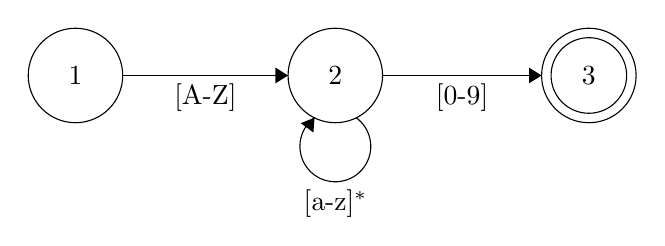
\begin{tikzpicture}[scale=0.2]
        \tikzstyle{every node}+=[inner sep=0pt]
        \draw [black] (22.9,-27) circle (3);
        \draw (22.9,-27) node {$1$};
        \draw [black] (39.4,-27) circle (3);
        \draw (39.4,-27) node {$2$};
        \draw [black] (55.5,-27) circle (3);
        \draw (55.5,-27) node {$3$};
        \draw [black] (55.5,-27) circle (2.4);
        \draw [black] (25.9,-27) -- (36.4,-27);
        \fill [black] (36.4,-27) -- (35.6,-26.5) -- (35.6,-27.5);
        \draw (31.15,-27.5) node [below] {[A-Z]};
        \draw [black] (42.4,-27) -- (52.5,-27);
        \fill [black] (52.5,-27) -- (51.7,-26.5) -- (51.7,-27.5);
        \draw (47.45,-27.5) node [below] {[0-9]};
        \draw [black] (40.723,-29.68) arc (54:-234:2.25);
        \draw (39.4,-34.25) node [below] {[a-z]$^*$};
        \fill [black] (38.08,-29.68) -- (37.2,-30.03) -- (38.01,-30.62);
    \end{tikzpicture}
\end{center}
\vspace{5mm}

Regular languages and, by extension, finite-state machines are often used in string searching algorithms. FSMs and regular languages are also often used in the lexical analysis (lexing) done by a compiler. That is, they give language designers the power to specify which words are valid in their programming language. \\

\subsection{Pushdown Automata}

Pushdown automata (PDA) are finite-state machines that also have access to a stack. These automata introduce a notion of \textit{history} or \textit{memory}. A PDA can push a symbol onto its stack on every transition, which will provide information in the future about actions in the past. It can also pop or peek at the stack to decide which transition to take next. \\

Pushdown automata can distinguish syntactically correct sentences from random sequences of valid words, something finite-state automata cannot do because they have no notion of what comes earlier than a given point in a given sentence. For example, a pushdown automaton would be able to tell that "my dog bites red toys" is a valid English sentence and "red my toys dog bites" is not. However, PDA cannot understand semantics. It would also consider "my dog \textit{barks} red toys" a valid English sentence, even though it has no meaning. \\

Pushdown automata can read \textit{context-free languages}, which are languages that follow a \textit{context-free grammar}. Context-free languages are formal languages whose production rules are of the form $A\rightarrow\alpha$ where $A$ is a nonterminal and $\alpha$ is a sequence that may contain terminals and nonterminals. A PDA pops terminals from its stack. When a nonterminal $A$ is at the top of the stack, the PDA can pop it and push the $\alpha$ of some production rule onto the stack. In a sense, the stack of the PDA contains the unprocessed data of the grammar. \\

Context-free grammars can be written to formalize languages such as the language of matching parentheses or the language of infix algebraic expressions (e.g. (2+4)/7*8). PDA and context-free languages are often used in the syntactic analysis (parsing) done by a compiler. That is, they give language designers the power to specify how valid sentences are structured in their programming language. \\

\subsection{Linear Bounded Automata}

Imagine that, instead of a stack, an automaton could have access to a finite-length list. Linear bounded automata (LBA) have a finite number of \textit{states}, a finite length of \textit{tape}, and a \textit{head} that can read and write symbols on the tape and move left or right along it, one symbol at a time. The length of the tape is a linear function of the length of the input, so we can say that the tape has $kn$ cells, where $n$ is the length of the input instructions and $k$ is a constant. \\

This machine is similar to the idea of a modern computer. The tape represents a finite amount of memory, and the head is able to read and write to it. LBA can understand \textit{context-sensitive languages}, which are languages that follow a \textit{context-sensitive grammar}. Sophisticated programming languages are context-sensitive, so a linear bounded automaton would be able to read and understand modern software. The $kn$-length tape acts as a sufficient environment for computationally demanding programming tasks, given a large enough $k$. Similarly, given enough memory, real computers can also solve very computationally difficult problems. \\

A context-sensitive language is a language where semantics matter. Using our earlier example, "my dog barks red toys" would not be a valid sentence in a context-sensitive version of English. An LBA then is actually able to differentiate data types and can tell when an operation is defined for one type and undefined for another. LBA and context-sensitive languages are often used in the semantic analysis (type checking) done by a compiler. That is, they give language designers the power to specify whether or not a syntactically correct sentence actually has any real \textit{meaning} in their programming language. \\

Where can we go from here? LBA are suitable models of real-world computers, and they can process semantic language. What more can we do? Let's try making the tape infinitely long$\dots$ \\

\subsection{Turing Machines}

A \textit{Turing machine} (TM) not only models real-world computers, but \textit{computation} itself. The concept, which was formalized in 1936 by Alan Turing, generalizes automata and defines the limitations of mechanical computing. It specifies a set of components that are necessary and sufficient for creating a "problem-solving machine" that is capable of solving any problem that can be solved by a machine. Weaker automata can solve \textit{some} of these machine-solvable problems, but only \textit{Turing-complete} automata (those that are functionally equivalent to TMs) have the expressive power to solve \textit{any} of them. The components of a Turing machine are listed below.

\begin{itemize}
    \item An infinitely long \textit{tape} that is divided into cells, each of which contains a symbol from some finite alphabet. One symbol from this alphabet is considered blank, and the tape is initially filled with these symbols.
    \item A \textit{head} that can read and write symbols on the tape and move left or right along it, one symbol at a time.
    \item A \textit{state register} that stores its current state and initially stores its starting state.
    \item A \textit{finite table of instructions} that, given the machine's current state and tape symbol, tells the machine to do the following sequence of actions:
    \begin{enumerate}
        \item Erase or write a symbol at the current tape cell (or do nothing)
        \item Move the head one tape cell to the left or right (or do nothing).
        \item Depending on the current state and input, transition to a different state (or the same state) or halt computation.
    \end{enumerate}
\end{itemize}

A machine like this need not be a real-world computer. In fact, in his original proof, \textit{On Computable Numbers, with an Application to the Entscheidungsproblem}, Turing refers to a person, whom he calls the "computer," as an example of a Turing machine. If we break down these components into the resources they represent, it becomes clear that many systems could be considered Turing machines.

\begin{itemize}
    \item The infinitely long tape represents \textit{infinite space for computation} or \textit{infinite memory}.
    \item The head represents three abilities:
        \begin{enumerate}
            \item Reading memory,
            \item Writing to memory,
            \item Traversing the memory freely, with no side effects.
        \end{enumerate}
    \item The state register represents the ability to \textit{know what "step" you are on} in the problem-solving process. We will clarify this ambiguous idea in a second, but for now just think of it as having an idea of your progress.
    \item The finite table of instructions represents a \textit{sequence of commands} or \textit{program} that can be followed unambiguously. The automaton can follow and obey these commands in order without any actual thought.
\end{itemize}

As long as you have unlimited space to work in, the freedom to read and write symbols anywhere in that space, a list of instructions to follow exactly, and the knowledge of what to do next, you have a Turing machine. We can now visualize the person Turing referred to as a "computer." It is a man with an infinitely large piece of paper, a pen that he writes symbols with, a list of instructions that tells him which symbols to write, where on the paper to move his pen tip, which instruction to perform next, and a knowledge of which instruction he is currently performing. Many systems of logic, such as programming languages, are Turing-complete. Many things not traditionally thought of as "systems of logic" are \underline{also Turing-complete}. \\\\

% https://www.toothycat.net/~hologram/Turing/index.html

\begin{tcolorbox}[breakable, enhanced, colback=textbook-blue, sharp corners]
    \vspace{3mm}
    \begin{center}
        \textbf{Turing Machines and Consciousness}
    \end{center}

    In 1950, Turing developed the \textit{Turing test}, a test of a machine's ability to exhibit behavior indistinguishable from that of a human. It involves an interrogator who is tasked with having two separate text conversations and determining which of the two participants is actually a machine. If the interrogator cannot distinguish a difference, the machine has passed the test. Despite its importance to the philosophy of computer science, the test is not a good indicator of whether or not a computer can think. The test says more about how gullible the interrogator is than how conscious the computer is. At the end of the day, the computer is still following its programming. \\
        
    What about this man whom Turing calls a "computer"? Would he pass the test, given the right programming? Perhaps he would. But that would not make him a \textit{person}. What kind of person is this man if he follows whatever instructions he is given? He is a slave, a person who always obeys. Could we say then that machines are also, in a certain sense of the word, slaves? Perhaps this is where the term \textit{master-slave technology} came from. Regardless, it is important to make a philosophical distinction here about what separates humans from machines or, more precisely, what distinguishes \textit{thought} from \textit{computation}. \\
        
    Essentially, this boils down to the question of consciousness. There is much debate about consciousness. Philosophers have proposed a variety of concepts that partially define it such as free will (the ability to choose) or qualia (the raw experience of existence, e.g. sounds, colors, emotions). However, \textit{intentionality} is one characteristic that is generally agreed upon as necessary for conscious thought. Intentionality is the ability of the mind to think \textit{about} something. Computers can \textit{think} things, but they cannot \textit{think about} things. They lack intentionality.\\
        
    For a Turing machine, the list of instructions is an essential component. It is capable of "thinking" if and only if some one tells it what to think. That effort is more accurately defined by the term "computation." We would also refer to the man's efforts with his pen and infinite paper as computations because they require no thought. If he were nothing more than a Turing machine, the man would not be able to perform mathematics on his own. In fact, he would not be able to do anything without instructions. It is the moment when he does something without being explicitly told to do it that he first displays consciousness. When \textit{unprompted} computation is performed for some \textit{purpose}, we can talk about consciousness. \\
        
    So calling computers slaves is a bit of an anthropomorphization. A slave is a conscious being who is forced to act like a machine. Computers don't have the prerequisite consciousness. No matter how complicated its architecture or sophisticated its artificial intelligence software, a computer is a \textit{tool} like a microwave or a calculator. Could it ever be more than that? Could a technology ever think? \underline{Perhaps}. But such a thing would be quite different from a Turing machine or any modern computer. \\

    % https://en.wikipedia.org/wiki/Artificial\_consciousness
        
    \parbreak
        
    \begin{displayquote}
        \textit{In attempting to construct such machines we should not be irreverently usurping His power of creating souls, any more than we are in the procreation of children: rather we are, in either case, instruments of His will providing mansions for the souls that He creates.}
        \vspace{4mm}
        \begin{flushright}
            ---Alan Turing (1950), \\
            in response to a theological objection to artificial consciousness.
        \end{flushright}
    \end{displayquote}

    \vspace{3mm}
\end{tcolorbox}
\vspace{2\baselineskip}

A single-tape Turing machine is formally defined as a septuple $(Q,\Gamma,b,\Sigma,\delta,q_0,F)$, where

\begin{itemize}
    \item $Q$ is a finite, non-empty set of \textit{states},
    \item $\Gamma$ is a finite, non-empty \textit{tape alphabet},
    \item $b\in\Gamma$ is the \textit{blank symbol},
    \item $\Sigma\subseteq\Gamma\setminus \{b\}$ is the set of symbols that can be written on the tape,
    \item $\delta$ is a partial function $\delta : (Q\setminus F)\times\Gamma\nrightarrow \Gamma\times\{L,R\}\times Q$ called the \textit{transition function}, which inputs the current state and tape symbol and outputs the symbol to write to the tape, the direction to move the head, and the next state to transition to,
    \item $q_0\in Q$ is the \textit{starting state}, and
    \item $F\subseteq Q$ is the set of \textit{final states}. The contents of the tape are \textit{accepted} if the Turing machine halts computation in a state from $F$.
\end{itemize}

We should now address what exactly "state" is in regard to computing. Many people associate it with the current instruction being fed to the machine. However, Turing made a distinction between this interpretation of state and the interpretation of state as the computer's "progress" or "state of mind." Turing's \textit{complete configuration} of state includes not only the current instruction, but the current symbol configuration of the entire tape as well and all the instructions yet to be executed. In this way, state is defined by the results of past instructions and the inevitable execution of future instructions. \\

Now we have defined what a Turing machine is, but it is still not clear why it is considered such a landmark concept in computer science. For example, if real-world computers can be sufficiently modeled by linear bounded automata, why do we instead focus so heavily on Turing machines? \\

Turing machines are the class of automata that can read \textit{recursively enumerable languages}. A formal language is called recursively enumerable, if it is a \textit{recursively enumerable subset} in the set of all possible words over the alphabet of the language. This essentially means that, for a language of this type, there exists an algorithm that can output a list of every word in the language. Consider what would be required for such an algorithm. How many valid words are there in a given language? Depending on its rules for constructing words, there may be an infinite amount. This is the case for some programming languages. A variable name could theoretically be as long as you want, provided you have enough memory to store it. In order to list all of the words in a recursively enumerable language, you would need infinite memory, which only a Turing machine can provide. \\

This does not imply that TMs can handle infinite lists of instructions. Rather, they can handle \textit{infinite looping} over a finite set of instructions. A Turing machine can "successfully" run a never-ending program. A real machine would use up all of its memory trying to run such a program, eventually crashing due to a \textit{stack overflow} (an attempt to write data outside of the limits of the memory). A TM would never run out of memory and, given infinite time, could run the program forever. \\

As previously stated, the Turing machine models not only computers, but \textit{computation}. It abstracts away the physical limitations of computers such as memory constraints, overheating, or hardware failure and asks what the fundamental limits of algorithmic computation are. It makes a statement on which mathematical problems are \textit{decidable}. It is an ideal computer, and, as such, it is not only a model of what real-world computers are today, but a model of what they \textit{could be} in the future, given sufficient advances in hardware. \\

\section{The Importance of Turing Machines to Modern Computing}

The automata we have discussed so far (finite-state machines, pushdown automata, linear bounded automata, and Turing machines) form a sort of hierarchy of machine capability. The formal grammars and languages that these automata can understand likewise constitute a hierarchy that was first described by Noam Chomsky in 1956. The \textit{Chomsky hierarchy}, a classification of the expressiveness of language according to grammatical rules, is summarized below by a table with columns for grammars, the languages those grammars build, and the class of automaton that can understand those languages.

\begin{table}[H]
    \caption{The Chomsky Hierarchy}
    \label{tab:LABEL}
    \begin{tabularx}{\textwidth}{|c|c|Y|}
        \vtabularspace{3}
        \hline
        Grammar & Language & Automaton \\
        \hline
        Type-0 & Recursively enumerable & Turing machine \\
        Type-1 & Context-sensitive & Linear bounded automaton \\
        Type-2 & Context-free & Pushdown automaton \\
        Type-3 & Regular & Finite-state machine \\
        \hline
        \vtabularspace{3}
    \end{tabularx}
\end{table}

As this is a hierarchy, higher-ranking automata are capable of doing anything that lower-ranking automata can. For example, an LBA can do anything that a PDA or FSM can and \textit{more}. To give a linguistic analogy, an LBA would be fluent in all of the languages that the PDA and FSM are fluent in, but would also be fluent in additional languages. What causes this difference in language facility? It is the structure of the automaton's memory. \\

Let's recap how these four automata handle memory.

\begin{itemize}
    \item An FSM has \textit{no} memory. It simply has a finite number of states, perhaps represented by a finite list of instructions. It can transition between states, but it has no notion of how it got to any particular state. It records no history.
    \item A PDA has a \textit{stack} of memory, but this form of memory is restricted. It cannot read or write its memory in any order it likes. It can read the top entry on the stack, but it must delete data to read entries located elsewhere.
    \item An LBA has a \textit{finite array} of memory. It can read or write this memory in any order it likes, but it has limitations on how much information it can store.
    \item A TM has an \textit{infinite array} of memory. It can read or write this memory in any order it likes, and it can also store as much as it likes.
\end{itemize}

It is no coincidence that real-world computers today use array-based memory. Arrays are both an intuitive and Turing-complete way to store information. Now, technically, LBA and TMs use "tape" instead of arrays, but the differences are minimal. In tape memory, cells have relative position, but they are not \textit{labeled}. Modern computers are actually modeled by \textit{register machines}. Register machines are equivalent in expressive power to Turing machines, but their memory is composed of an infinite-length array of uniquely addressed \textit{registers}. Like a tape of cells, an array of registers can be freely accessed. \\

A subset of register machines known as \textit{random-access machines} allow for \textsc{jump} instructions (e.g. jump to register \#5623) in addition to standard sequential traversal of memory (e.g. move right, move right, move right, etc). This allows computers to accomplish a task with fewer instructions, but the expressive powers of random-access machines and Turing machines are equivalent because both are capable of \textit{eventually} solving the task. Modern computers can be described as random-access machines because they use \textit{random-access memory} (RAM). In RAM, the time to access information is independent of physical location. From a performance perspective, this means that we do not have to consider \textit{where} we store things in memory. It's all uniformly fast. This allows for the construction of \textit{node-based} data structures, which we will discuss in a later section. \\\\

\begin{tcolorbox}[breakable, enhanced, colback=textbook-blue, sharp corners]    
    \vspace{3mm}
    \begin{center}
        \textbf{Exploring Exotic Automata}
    \end{center}

    It is worth thinking about automata whose memory is modeled by non-list data structures. For example, a pushdown automaton uses a stack to model its memory and because of this, it is not Turing-complete. What if it used a queue instead? In this case, it would be Turing-complete because it could dequeue items to traverse the memory and then enqueue them to avoid data loss. One could envision this as a Turing machine whose infinite tape ends are glued together to form an infinite loop. The machine can only move in one direction, but it can still access every cell because its tape is circular. \\
        
    The memory can also be modeled by non-sequential data structures to create some bizarre models of computation. What if the memory of a computer was laid out not as an array, but as an undirected tree? What if it was organized according to an algebraic structure like a monoid or a ring? I'm not even going to pretend that I understand what kind of behavior this would result in. But it is an \underline{area of active research}. \\

    % https://kluedo.ub.uni-kl.de/frontdoor/index/index/docId/4400

    Other tweaks can be made to the properties of a Turing machine to create new, interesting automata. For example, \textit{$\omega$-automata} (or \textit{stream automata}) are Turing machines that expect an \textit{infinite} sequence of instructions. \textit{$\omega$-automata} never stop running because an infinite sequence of instructions requires an infinite sequence of instruction executions. Because they never terminate, they never move into acceptance (final) states. Rather than a set of final states $F$, they have a set of \textit{acceptance conditions} $Acc$. \\
        
    For ordinary automata, every \textit{run} $\rho$ (i.e. a sequence of $n$ states) ends with a state $r_n$, and the input is only accepted if this state is final (i.e. $r_n\in F$). For $\omega$-automata, runs are infinite sequences, so they do not end with a state $r_n$ at all. How do we tell if a run $\rho$ should be accepted as a valid set of instructions? We require that $\rho\in Acc$. That is, if the run is a member of the "set of acceptable runs," it should be accepted. What is the "set of acceptable runs"? That depends on which variant of $\omega$-automaton you are talking about. \\
        
    The class of $\omega$-automata contains multiple automata with different definitions of $Acc$. For example, for some subset $F$ (final states) of $Q$ (all states), the \textit{B\"{u}chi automaton} accepts those runs $\rho$, for which there exists a final state that occurs "infinitely often" in $\rho$. What is a state that is visited "infinitely often"? Given an infinite amount of runtime, some states in $Q$ will be visited an infinite amount of times, and others will not. For example, what if you can transition away from your starting state $q_0$, but you are not allowed to transition into it. Even given infinite time, $q_0$ would not be visited infinitely often, and if it were the only state in $F$, you would never be able to construct a run that would be considered valid by a B\"{u}chi automaton. Nondeterministic B\"{u}chi automata have applications in "always-on" or "always listening" software, such as those used in highly-autonomous robots or smart speakers like the Amazon Echo, both of which receive instructions based on a never-ending, real-time stream of sensory data. \\
        
    Wow, that's a lot of abstract mathematics. Why is any of this important for gaining a fundamental understanding of Turing machines or real-world computers? It is important because we can only really grasp their \textit{scope} if we explore outside of it. Some automata can have properties that are not practical or possible to implement in the real-world. Mathematically, they could have infinite states or continuous alphabets or hyperdimensional memory. But here, once and for all, let's define the scope of computation we will be considering for the rest of this guide. \\
        
    A modern computer has:
        
    \begin{itemize}
        \item A \textbf{finite} set of states Q. If it were instead infinite, the automaton would have a state for every possible input, and thus would be able to understand any conceivable language. This is far too powerful a machine to build. This would essentially be a universal problem solver.
        \item A \textbf{finite} alphabet $\Sigma$. If it were instead infinite, the automaton could have a continuous alphabet. What kind of alphabet's symbols exist on a spectrum? Perhaps you could call \textit{sound} a "language" with a continuous alphabet known as frequency. An automaton with an infinite alphabet would not be digital and would not use bits. It would be an analog computer. Analog computers do exist, and they were popular in the 1950s and 1960s, but nowadays we write software for digital computers. \textit{Fun fact:} analog synthesizers, which are still commonly used in electronic music, are considered a kind of analog computer.
        \item A transition \textbf{function} $\delta$. If it were instead a relation (i.e. inputs are mapped to more than one output), the automaton would be nondeterministic. It is suspected that nondeterministic Turing machines would be able to solve NP-complete problems, which is a computational feat that has not yet been accomplished in a tractable way by a deterministic Turing machine.
    \end{itemize}

    \vspace{3mm}        
\end{tcolorbox}
\vspace{2\baselineskip}

While more exotic memory structures are theoretically possible, real-world computers use \textit{arrays} of memory. Since Turing machines can solve any computable problem and data structures are used by computers to solve problems, it follows that data structures can be simulated by Turing machines. Because register machines use array-based memory and are Turing-equivalent, it also follows that \textbf{all data structures can be implemented using arrays}. This is a very useful insight, and it will be discussed further in Section 3. \\

The selection of Turing machines (or register machines) as the model for real-world computers has also influenced decisions in computer architecture. In early computers, the instructions were not integrated into the machine. Code was written on punch cards, which were fed into computers. Eventually, code was stored digitally in programs that were uploaded to the computer's memory. This type of machine is known as a \textit{stored-program computer}. \\

Where should one store instructions or code in a stored-program computer? Those that have a \textit{Harvard architecture} store their instructions in an \textit{instruction memory} that is separate from the \textit{data memory}. Those that have a \textit{von Neumann architecture} store their instructions and data in the same physical memory, but partition the memory somehow to avoid overwriting the instructions. The von Neumann architecture allows "programs that write programs," such as assemblers, compilers, linkers, and loaders. Modern computers are more von Neumann than they are Harvard because their instructions and data share an address space, but they are not strictly either. We can describe modern computers as \textit{random-access stored-program} (RASP) machines with \textit{split-cache modified Harvard architectures}. \\

